\chapter{Recursive Data Types}\label{recursive_data_chap}

\emph{Recursive data types}%
\index{recursive data type|textbf}
%\index{recursive data type|seealso{induction}} 
play a central role in programming, and induction is really all about them.

Recursive data types are specified by \emph{recursive definitions},
which say how to construct new data elements from previous ones.
Along with each recursive data type there are recursive definitions of
properties or functions on the data type.  Most importantly, based on
a recursive definition, there is a \emph{structural induction}%
\index{induction!structural induction}
method for proving that all data of the given type have some property.

This chapter examines a few examples of recursive data types and
recursively defined functions on them:
\begin{itemize}
\item strings of characters,
\item ``balanced'' strings of brackets,
\item the nonnegative integers, and
\item arithmetic expressions.
\item two-player games with perfect information.
\end{itemize}

%\hyperdef{paren}{string}
\section{Recursive Definitions and Structural Induction}

We'll start off illustrating recursive definitions and proofs using
the example of character strings.  Normally we'd take strings of
characters for granted, but it's informative to treat them as a
recursive data type.  In particular, strings are a nice first example
because you will see recursive definitions of things that are easy to
understand, or that you already know, so you can focus on how the
definitions work without having to figure out what they are supposed
to mean.

Definitions of recursive data types have two parts:
\begin{itemize}
\item \inductioncase{Base case(s)} specifying that some known
  mathematical elements are in the data type, and
\index{base case|see{recursive data type}}

\item \inductioncase{Constructor case(s)} that specify how to construct new data
  elements from previously constructed elements or from base elements.
\end{itemize}

The definition of strings over a given character set $A$ follows this
pattern:

\begin{definition}\label{recstring_def}
  Let $A$ be a nonempty set called an \emph{alphabet}, whose elements
  are referred to as \emph{characters} (also called \emph{letters},
  \emph{symbols}, or \emph{digits}).  The recursive data type
  $\strings{A}$ of strings over alphabet $A$ is defined as follows:
\begin{itemize}
\item \inductioncase{Base case}: the empty string $\emptystring$ is in $\strings{A}$.

\item \inductioncase{Constructor case}: If $a \in A$ and $s \in \strings{A}$, then the pair
       $\ang{a,s} \in \strings{A}$.
\end{itemize}
\end{definition}
So $\strings{\set{0,1}}$ are the binary strings.

The usual way to treat binary strings is as sequences of 0's and 1's.
For example, we have identified the length-4 binary string 1011 as a
sequence of bits, the 4-tuple $(1,0,1,1)$.  But according to
the recursive Definition~\ref{recstring_def}, this string would be
represented by nested pairs, namely
\[
\ang{1,\ang{0,\ang{1,\ang{1,\emptystring}}}}.
\]
These nested pairs are definitely cumbersome and may also seem
bizarre, but they actually reflect the way that such lists of
characters would be represented in programming languages like Scheme
or Python, where $\ang{a,s}$ would correspond to $\text{cons}(a, s)$.

Notice that we haven't said exactly how the empty string is
represented.  It really doesn't matter, as long as we can recognize
the empty string and not confuse it with any nonempty string.

\begin{editingnotes}
Even before func def, define binary relation def, say ``$t$ a proper
suffix of $s''$ or ``$t$ is a subsequence of $s$'' and then set up
func def as special case
\end{editingnotes}

Continuing the recursive approach, let's define the length of a string.
\begin{definition}
The length $\lnth{s}$ of a string $s$ is defined recursively based
on Definition~\ref{recstring_def}.

\item \inductioncase{Base case}:  $\lnth{\emptystring} \eqdef\ 0$.

\item \inductioncase{Constructor case}: $\lnth{\ang{a,s}} \eqdef\ 1 + \lnth{s}$.

\end{definition}

This definition of length follows a standard pattern: functions on
recursive data types can be defined recursively using the same cases
as the data type definition.  Specifically, to define a function $f$
on a recursive data type, define the value of $f$ for the base cases
of the data type definition, then define the value of $f$ in each
constructor case in terms of the values of $f$ on the component data
items.

Let's do another example: the \emph{concatenation} $s\cdot t$ of the
strings $s$ and $t$ is the string consisting of the letters of $s$
followed by the letters of $t$.  This is a perfectly clear
mathematical definition of concatenation (except maybe for what to do
with the empty string), and in terms of Scheme/Python lists, $s\cdot
t$ would be the list $\text{append}(s, t)$.  Here's a recursive
definition of concatenation.

\begin{definition}\label{concat_def}
The \term{concatenation} $s\cdot t$ of the strings $s,t \in
\strings{A}$ is defined recursively based on
Definition~\ref{recstring_def}:

\item \inductioncase{Base case}:     % ($s=\emptystring$):
\[
\emptystring \cdot t \eqdef\ t.
\]

\item \inductioncase{Constructor case}: %($s = \ang{a,r}$ for $r \in \strings{A}$):
\[
\ang{a,s} \cdot t \eqdef\ \ang{a, s \cdot t}.
\]
\end{definition}

\subsection{Structural Induction}

\emph{Structural induction}%
\index{induction!structural induction|textbf} 
is a method for proving that all the elements
of a recursively defined data type have some property.  A structural
induction proof has two parts corresponding to the recursive definition:
\begin{itemize}
\item Prove that each base case element has the property.
\item Prove that each constructor case element has the property, when
  the constructor is applied to elements that have the property.
\end{itemize}

For example, in the base case of the definition of
concatenation~\ref{concat_def}, we \emph{defined} concatenation so the
empty string was a ``left identity,'' namely, $\emptystring \cdot
s\ \eqdef s$.  We want the empty string also to be ``right identity,''
namely, $s \cdot \emptystring = s$.  Being a right identity is not
part of Definition~\ref{concat_def}, but we can prove it easily by
structural induction:
\begin{lemma}\label{rightidempty}
\[
s \cdot \emptystring = s
\]
for all $s \in \strings{A}$.
\end{lemma}

\begin{proof}
The proof is by structural induction on the recursive
definition~\ref{concat_def} of concatenation.  The induction
hypothesis will be
\[
P(s) \eqdef\ [s \cdot \emptystring = s].
\]

\inductioncase{Base case}: ($s = \emptystring$).
\begin{align*}
s \cdot \emptystring
    & = \emptystring \cdot \emptystring\\
    & = \emptystring
        & \text{($\emptystring$ is a left identity by Def~\ref{concat_def})}\\
    & = s.
\end{align*}

\inductioncase{Constructor case}: ($s = a \cdot t$).
\begin{align*}
s \cdot \emptystring
   & =(a \cdot t) \cdot \emptystring\\
   & = a \cdot (t \cdot \emptystring)
       & \text{(Constructor case of Def~\ref{concat_def})}\\
   & = a \cdot t
        & \text{by induction hypothesis $P(t)$}\\
   & = s.
\end{align*}
So $P(s)$ holds.  This completes the proof of the constructor case,
and we conclude by structural induction that
equation~\eqref{rightidempty} holds for all $s \in \strings{A}$.
\end{proof}

We can also verify properties of recursive functions by structural
induction on their definitions.  For example, let's verify the
familiar fact that the length of the concatenation of two strings is
the sum of their lengths:

%\begin{theorem}\label{stAl+}
%\end{theorem}
\begin{lemma*}
\[
\lnth{s\cdot t} = \lnth{s} + \lnth{t}
\]
for all $s,t \in \strings{A}$.
\end{lemma*}

\begin{proof}
By structural induction on the definition of $s \in \strings{A}$.   The
induction hypothesis is
\[
P(s) \eqdef\ \forall t \in \strings{A}.\, \lnth{s\cdot t} = \lnth{s} + \lnth{t}.
\]

\inductioncase{Base case} ($s = \emptystring$):
\begin{align*}
\lnth{s \cdot t}
   & = \lnth{\emptystring \cdot t}\\
   & = \lnth{t}
         & \text{(base case of Def~\ref{concat_def} of concatenation)}\\
   & = 0 + \lnth{t}\\
   & = \lnth{s} + \lnth{t}
         & \text{(Def of $\lnth{\emptystring}$)}.
\end{align*}

\inductioncase{Constructor case}: ($s \eqdef \ang{a,r}$).
\begin{align*}
\lnth{s \cdot t}
    & = \lnth{\ang{a, r} \cdot t}\\
    & = \lnth{\ang{a,r \cdot t}}
        &  \text{(constructor case of Def of concat)}\\
    & = 1 + \lnth{r \cdot t}
        &  \text{(constructor case of def length)}\\
    & = 1 +  (\lnth{r} + \lnth{t})
        & \text{(ind. hyp. $P(r)$)}\\
    & = (1 +  \lnth{r}) + \lnth{t}\\
    & = \lnth{\ang{a,r}} + \lnth{t}
        & \text{(constructor case, def of length)}\\
    & = \lnth{s} + \lnth{t}.
\end{align*}
This proves that $P(s)$ holds, completing the constructor case.  By
structural induction, we conclude that $P(s)$ holds for all strings $s
\in \strings{A}$.
\end{proof}

These proofs illustrate the general principle:

\textbox{ 
\textboxtitle{The Principle of Structural Induction.}

Let $P$ be a predicate on a recursively defined data type $R$.  If
%
\noindent \begin{itemize}
\item $P(b)$ is true for each base case element $b \in R$, and

\item for all two-argument constructors $\mathbf{c}$,
\[
[P(r)\QAND P(s)] \QIMPLIES P(\mathbf{c}(r, s))
\]
for all $r,s \in R$,\\
and likewise for all constructors taking other numbers of arguments,
\end{itemize}
then
\[
P(r) \text{ is true for all } r \in R.
\]
}

\begin{problems}
\practiceproblems
\pinput{FP_binary_tree_induction}

\classproblems
\pinput{CP_string_associativity}
\pinput{CP_string_reversal}
\pinput{CP_F18_functions}
\pinput{CP_recursively_defined_sets}
\pinput{CP_binary_trees}

\homeworkproblems
%\pinput{PS_string_cancellation}
\pinput{PS_palindromes}
\pinput{PS_linear_combination_by_structural_induction}
\pinput{PS_count_a_s_lem}
\pinput{PS_koch_snowflake}
\pinput{PS_red_black_tree_induction}

\examproblems
\pinput{FP_arith_trig_functions}
\pinput{FP_structural_induction_rational_composition_s16}
\pinput{FP_structural_linear_product}
\pinput{FP_recstrings}

%%%%\pinput{CP_recursive_binary_trees}  %%problem idea, needs work.
\end{problems}

\section{Strings of Matched Brackets}

Let $\brkts$ be the set of all strings of square brackets.  For example,
the following two strings are in $\brkts$:
\begin{equation}\label{2strings}
\lefbrk\rhtbrk\rhtbrk\lefbrk\lefbrk\lefbrk\lefbrk\lefbrk\rhtbrk\rhtbrk\quad \text{and}\quad \lefbrk\lefbrk\lefbrk\rhtbrk\rhtbrk\lefbrk\rhtbrk\rhtbrk\lefbrk\rhtbrk
\end{equation}

A string $s \in \brkts$ is called a \emph{matched string} if its
brackets ``match up'' in the usual way.  For example, the left-hand
string above is not matched because its second right bracket does not
have a matching left bracket.  The string on the right is matched.

We're going to examine several different ways to define and prove
properties of matched strings using recursively defined sets and
functions.  These properties are pretty straightforward, and you might
wonder whether they have any particular relevance in computer science.
The honest answer is ``not much relevance \emph{any more}.''  The reason
for this is one of the great successes of computer science, as explained in
the text box below.

\textbox{
\textboxheader{Expression Parsing}
%Flesh this out and get references

During the early development of computer science in the 1950's and 60's,
creation of effective programming language compilers was a central
concern.  A key aspect in processing a program for compilation was
expression parsing.  One significant problem was to take an expression
like
\[
x + y * z^2 \div y + 7
\]
and \emph{put in} the brackets that determined how it
should be evaluated---should it be
\begin{align*}
[[x + y] * z^2 \div y] + 7,\text{ or}, \\
x + [y * z^2 \div [y + 7]], \text{ or},\\
[x + [y * z^2 ]] \div [y + 7], \text{ or}\dots?
\end{align*}

The Turing award (the ``Nobel Prize'' of computer science) was
ultimately bestowed on Robert W. Floyd,%
\index{Floyd, Robert W.} 
for, among other things,
discovering simple procedures that would insert the brackets properly.

In the 70's and 80's, this parsing technology was packaged into high-level
compiler-compilers that automatically generated parsers from expression
grammars.  This automation of parsing was so effective that the subject no
longer demanded attention.  It had largely disappeared from the computer
science curriculum by the 1990's.}

\iffalse
One precise way to determine if a string is matched is to start with 0 and
read the string from left to right, adding 1 to the count for each left
bracket and subtracting 1 from the count for each right bracket.
For example, here are the counts for the two strings above
\[\begin{array}{rrrrrrrrrrrrr}
& \lefbrk & \rhtbrk & \rhtbrk & \lefbrk & \lefbrk & \lefbrk & \lefbrk &
\lefbrk & \rhtbrk & \rhtbrk & \rhtbrk & \rhtbrk\\
0 & 1 & 0 & -1 & 0 & 1 & 2 & 3 & 4 & 3 & 2 & 1 & 0\\
\\
\\
& \lefbrk & \lefbrk & \lefbrk & \rhtbrk & \rhtbrk & \lefbrk & \rhtbrk &
\rhtbrk & \lefbrk & \rhtbrk\\
0 & 1 & 2 & 3 & 2 & 1 & 2 & 1 & 0 & 1 & 0
\end{array}\]
A string has a \emph{good count} if its running count never goes
negative and ends with 0.  So the second string above has a good count, but
the first one does not because its count went negative at the third step.
\begin{definition}\label{gc-def}
Let
\[
\GC \eqdef\  \set{ s \in \brkts \suchthat s\ \text{has a good count}}.
\]
\end{definition}
The matched strings can now be characterized precisely as this set of
strings with good counts.
\fi

The matched strings can be nicely characterized as a recursive data type:

\begin{definition}\label{RM_def}\label{RM-def}
Recursively define the set $\RM$ of strings as follows:
\begin{itemize}

\item \inductioncase{Base case}: $\emptystring \in\RM$.

\item \inductioncase{Constructor case}: If $s,t \in\RM$, then
\[
\lefbrk s\, \rhtbrk t \in \RM.
\]
\end{itemize}

\end{definition}

Here $\lefbrk s\, \rhtbrk t$ refers to the concatenation of
strings which would be written in full as
\[
\lefbrk \cdot (s \cdot (\rhtbrk \cdot t)).
\]
From now on, we'll usually omit the ``$\cdot$'s.'' 

Using this definition, $\emptystring \in\RM$ by the base
case, so letting $s=t =\emptystring$ in the constructor case implies
\[
\lefbrk\emptystring\rhtbrk\emptystring=\lefbrk\rhtbrk\in\RM.
\]
Now,
\begin{align*}
\lefbrk\emptystring\rhtbrk\lefbrk\rhtbrk &= \lefbrk\rhtbrk\lefbrk\rhtbrk \in \RM
    & \text{(letting $s = \emptystring, t = \lefbrk\rhtbrk$)}\\
\lefbrk\lefbrk\rhtbrk\rhtbrk\emptystring & = \lefbrk\lefbrk\rhtbrk\rhtbrk \in \RM
    & \text{(letting $s = \lefbrk\rhtbrk, t = \emptystring$)}\\
&\ \ \lefbrk\lefbrk\rhtbrk\rhtbrk\lefbrk\rhtbrk \in \RM
    & \text{(letting $s = \lefbrk\rhtbrk, t = \lefbrk\rhtbrk$)}
\end{align*}
are also strings in $\RM$ by repeated applications of the constructor
case; and so on.

\iffalse
If you haven't seen this kind of definition before, you should
try continuing this example to verify that
$\lefbrk\lefbrk\lefbrk\rhtbrk\rhtbrk\lefbrk\rhtbrk\rhtbrk\lefbrk\rhtbrk
\in \RM$.
\fi


\iffalse
Given the way this section is set up you might guess that $\RM = \GC$,
and you'd be right, but it's not completely obvious.  The proof is worked
out in Problem~\ref{PS_bracket_good_count}.
\fi

It's pretty obvious that in order for brackets to match, there had
better be an equal number of left and right ones.  For further
practice, let's carefully prove this from the recursive definitions,
beginning with a recursive definition of the number $\cnt{c}{s}$ of
occurrences of the character $c \in A$ in a string $s$:

\begin{definition}\label{countas_def} \mbox{}

\inductioncase{Base case}: $\cnt{c}{\emptystring} \eqdef\ 0$.

\inductioncase{Constructor case}:
\[
\cnt{c}{\ang{a,s}} \eqdef \begin{cases}
                           \cnt{c}{s}  &\text{ if } a \neq c,\\
                           1 + \cnt{c}{s} &\text{ if } a = c.
                           \end{cases}
\]
\end{definition}

The following Lemma follows directly by structural induction on
Definition~\ref{countas_def}.  We'll leave the proof for practice
(Problem~\ref{PS_count_a_s_lem}).

\begin{lemma}\label{countas_lem}
\[
\cnt{c}{s \cdot t} = \cnt{c}{s} + \cnt{c}{t}.
\]
\end{lemma}

\begin{lemma*}
Every string in $\RM$ has an equal number of left and right brackets.

\begin{proof}
The proof is by structural induction with induction hypothesis
\[
P(s) \eqdef\  \brac{\cnt{\lefbrk}{s} = \cnt{\rhtbrk}{s}}.
\]

\inductioncase{Base case}: $P(\emptystring)$ holds because
\[
\cnt{\lefbrk}{\emptystring} = 0 = \cnt{\rhtbrk}{\emptystring}
\]
by the base case of Definition~\ref{countas_def} of $\cnt{c}{}$.

\inductioncase{Constructor case}: By structural induction hypothesis, we assume
$P(s)$ and $P(t)$ and must show $P(\lefbrk s\,\rhtbrk t)$:
\begin{align*}
\cnt{\lefbrk}{\lefbrk s\,\rhtbrk t}
    & = \cnt{\lefbrk}{\lefbrk} + \cnt{\lefbrk}{s}
        +\cnt{\lefbrk}{\rhtbrk}+ \cnt{\lefbrk}{t}
         & \text{(Lemma~\ref{countas_lem})}\\
    & = 1 + \cnt{\lefbrk}{s} + 0 + \cnt{\lefbrk}{t}
         & \text{(def $\cnt{\lefbrk}{}$)}\\
    & = 1 + \cnt{\rhtbrk}{s} + 0 + \cnt{\rhtbrk}{t}
         & \text{(by $P(s)$ and $P(t)$)}\\
    & = 0 + \cnt{\rhtbrk}{s} + 1 + \cnt{\rhtbrk}{t}\\
    & = \cnt{\rhtbrk}{\lefbrk} + \cnt{\rhtbrk}{s}
        +\cnt{\rhtbrk}{\rhtbrk}+ \cnt{\rhtbrk}{t}
         & \text{(def $\cnt{\rhtbrk}{}$)}\\
    & = \cnt{\rhtbrk}{\lefbrk s\,\rhtbrk t}
            & \text{(Lemma~\ref{countas_lem})}
\end{align*}
This completes the proof of the constructor case.  We conclude by
structural induction that $P(s)$ holds for all $s \in\RM$.
\end{proof}
\end{lemma*}

\iffalse

The \term{depth} of a matched string is defined recursively as follows
\begin{definition}
The \emph{depth} $d(s)$ of a string $s \in\RM$ is defined
recursively by the rules:
\begin{itemize}
\item $d(\emptystring) \eqdef\  0.$
\item $d(\lefbrk s\,\rhtbrk t)
    \eqdef\ \max \set{d(s) + 1, d(t)}$
\end{itemize}
\end{definition}
\fi

\textbf{Warning:}%
\index{recursive data type!ambiguity} 
When a recursive definition of a data type allows
the same element to be constructed in more than one way, the
definition is said to be \emph{ambiguous}.  We were careful to choose
an \emph{un}ambiguous definition of $\RM$ to ensure that functions
defined recursively on its definition would always be well-defined.
Recursively defining a function on an ambiguous data type
definition usually will not work.  To illustrate the problem, here's
another definition of the matched strings.

\iffalse Recursive definitions of tagged data types, where the tag
uniquely determines the rule used to construct an element, are guaranteed
to be unambiguous.
\fi

\begin{definition}
\label{AM_def}
Define the set, $\AM \subseteq \brkts$ recursively as follows:
\begin{itemize}

\item \inductioncase{Base case}: $\emptystring \in \AM$,

\item \inductioncase{Constructor cases}: if $s,t \in \AM$, then
  the strings $\lefbrk s\, \rhtbrk$ and $st$ are also in $\AM$.
\end{itemize}
\end{definition}

It's pretty easy to see that the definition of $\AM$ is just another way
to define $\RM$, that is $\AM = \RM$ (see Problem~\ref{PS_RM_equal_AM}).
The definition of $\AM$ is arguably easier to understand, but we didn't
use it because it's ambiguous, while the trickier definition of $\RM$ is
unambiguous.  Here's why this matters.  Let's define the number of
operations $f(s)$ to construct a matched string $s$ recursively on the
definition of $s \in \AM$:
\begin{align*}
  f(\emptystring)        & \eqdef\ 0, \tag{$f$ base case}\\
  f(\lefbrk s\,\rhtbrk\ ) & \eqdef\ 1+ f(s), \\
  f(st)                  & \eqdef\ 1+ f(s) +f(t).\tag{$f$ concat case}
\end{align*}
This definition may seem ok, but it isn't:
$f(\emptystring)$ winds up with two values, and consequently:
\begin{align*}
0 & = f(\emptystring) & \text{($f$ base case))}\\
  & = f(\emptystring \cdot \emptystring) & \text{(concat def, base case)} \\
                & = 1 + f(\emptystring) + f(\emptystring)
                      &  \text{($f$ concat case)},\\
                & = 1 + 0 + 0 = 1
                      & \text{($f$ base case)}.
\end{align*}
This is definitely not a situation we want to be in!


\iffalse

Now suppose $s = \lefbrk\rhtbrk\lefbrk\rhtbrk\lefbrk\rhtbrk\lefbrk\rhtbrk$.


%%FIND SIMPLER EXAMPLE

Let $a$ be the string $\lefbrk\lefbrk\rhtbrk\rhtbrk \in M$ built by two successive
applications of the first $M$ constructor starting with $\emptystring$.  Next
let $b \eqdef aa$ and $c \eqdef bb$, each built by successive applications
of the second $M$ constructor.

Alternatively, we can build $ba$ from the second constructor with $s=b$
and $t=a$, and then get to $c$ using the second constructor with $s=ba$
and $t=a$.

Now by these rules, $f(a) = 2$ and $f(b) = (2+1)(2+1)=9$.  This means
that $f(c) = f(bb)= (9+1)(9+1)=100$.

But also $f(ba) = (9+1)(2+1) = 27$, so that $f(c) = f(ba\,a) = (27 +1)
(2+1) = 84$.

The outcome is that $f(c)$ is defined to be both 100 and 84, which shows
that the rules defining $f$ are inconsistent.

On the other hand, structural induction remains a sound proof method even
for ambiguous recursive definitions, which is why it is easy to prove
that $M=\RM$.
\fi

\begin{problems}

\practiceproblems
\pinput{MQ_recursive_power5}
\pinput{MQ_ambiguous_recursive_def}

\classproblems
\pinput{CP_erasable_strings}
\pinput{PS_RM_equal_AM}

\homeworkproblems
\pinput{PS_bracket_good_count}
\pinput{CP_triangle_tiling_recursive}
\pinput{PS_starfree_recursive}
\pinput{PS_circuit_data_type}

\examproblems
\pinput{CP_XOR_AND_recursive}
\end{problems}

\section{Recursive Functions on Nonnegative Integers}

The nonnegative integers can be understood as a recursive data type.
\begin{definition}\label{0succ}
The set $\nngint$ is a data type defined recursively as:
\begin{itemize}
\item $0 \in \nngint$.
\item If $n \in \nngint$, then the \emph{successor} $n+1$ of $n$ is in
$\nngint$.
\end{itemize}

\end{definition}

The point here is to make it clear that ordinary induction is simply the
special case of structural induction on the recursive
Definition~\ref{0succ}.  This also justifies the familiar recursive
definitions of functions on the nonnegative integers.

\subsection{Some Standard Recursive Functions on $\nngint$}

\begin{example}\label{factorial-def}

\emph{The factorial%
\index{factorial|textbf} function.}  This function is often written
``$n!$.''  You will see a lot of it in later chapters.  Here, we'll use
the notation $\text{fac}(n)$:
\begin{itemize}
\item $\text{fac}(0) \eqdef 1$.
\item $\text{fac}(n+1) \eqdef (n+1)\cdot \text{fac}(n)$ for $n \ge 0$.
\end{itemize}
\end{example}

\begin{example}
\emph{Summation notation.}\label{sum-notation-def}\index{summation notation} Let 
``$S(n)$'' abbreviate the expression ``$\sum_{i=1}^n f(i)$.''  We can recursively define
$S(n)$ with the rules
  \begin{itemize}
  \item $S(0) \eqdef 0$.
  \item $S(n+1) \eqdef  f(n+1) + S(n)$ for $n\geq 0$.
  \end{itemize}
\end{example}

\begin{editingnotes}

\item[Simultaneous recursive definitions:]
  You can define several things at the same time, in terms of each
  other.  For example, we may define two functions $f$ and $g$ from
  $\nngint$ to $\nngint$, recursively, by:
  \begin{itemize}
  \item
    $f(0) \eqdef 1$,
  \item
    $g(0) \eqdef 1$,
  \item
    $f(n+1) \eqdef f(n) + g(n)$, for $n \geq 0$,
  \item
    $g(n+1) \eqdef f(n) \cdot g(n)$, for $n \geq 0$.
  \end{itemize}

\end{editingnotes}

\begin{editingnotes}

\subsection{Induction on Fibonacci Numbers}

We can use the recursive definition of a function to establish its
properties by structural induction.

As an illustration, we'll prove a cute identity involving Fibonacci
numbers.  Fibonacci numbers provide lots of fun for mathematicians because
they satisfy many such identities.
\begin{proposition}
\[
\forall n \geq 0 (\Sigma_{i=0}^n F_i^2 = F_n F_{n+1}).
\]
\end{proposition}

Example: $n = 4$:
\[
0^2 + 1^2 + 1^2 + 2^2 + 3^2 = 15 = 3 \cdot 5.
\]
Let's try a proof by (ordinary, not strong) induction.  The theorem
statement suggests trying it with $P(n)$ defined as:
\[
\sum_{i=0}^n F_i^2 = F_n F_{n+1}.
\]

\inductioncase{Base case} ($n=0$):
$\Sigma_{i=0}^0 F_i^2 \eqdef (F_0)^2 = 0 = F_0 F_1$ because
$F_0 \eqdef 0$.

\inductioncase{Inductive step} ($n\geq 0$): Now we stare at the gap
between $P(n)$ and $P(n+1)$.  $P(n+1)$ is given by a summation that's
obtained from that for $P(n)$ by adding one term; this suggests that,
once again, we subtract.  The difference is just the term $F_{n+1}^2$.
Now, we are assuming that the original $P(n)$ summation totals $F_n
F_{n+1}$ and want to show that the new $P(n+1)$ summation totals
$F_{n+1} F_{n+2}$.  So we would \emph{like} the difference to be
\[
F_{n+1} F_{n+2} - F_n F_{n+1}.
\]

So, the actual difference is $F_{n+1}^2$ and the difference we want is
$F_{n+1} F_{n+2} - F_n F_{n+1}$.  Are these the same?  We want to check
that:
\[
F_{n+1}^2 = F_{n+1} F_{n+2} - F_n F_{n+1}.
\]
But this is true, because it is really the Fibonacci definition in
disguise: to see this, divide by $F_{n+1}$.

\end{editingnotes}

\subsection{Ill-formed Function Definitions}
%\hyperdef{ill}{formed}

There are some other blunders to watch out for when defining functions
recursively.  The main problems come when recursive definitions don't
follow the recursive definition of the underlying data type.  Below are
some function specifications that resemble good definitions of functions
on the nonnegative integers, but really aren't.

\begin{eqnarray}\label{f1}
f_1(n)\eqdef 2+f_1(n-1).
\end{eqnarray}
This ``definition'' has no base case.  If some function $f_1$
satisfied~(\ref{f1}), so would a function obtained by adding a constant to
the value of $f_1$.  So equation~(\ref{f1}) does not uniquely define
an $f_1$.

\begin{eqnarray}\label{f2}
f_2(n) \eqdef
\begin{cases}
 0, & \text{if $n=0$},\\
 f_2(n+1) &  \text{otherwise}.
\end{cases}
\end{eqnarray}
This ``definition'' has a base case, but still doesn't uniquely determine
$f_2$.  Any function that is 0 at 0 and constant everywhere else would
satisfy the specification, so~\eqref{f2} also does not uniquely define
anything.

In a typical programming language, evaluation of $f_2(1)$ would begin with
a recursive call of $f_2(2)$, which would lead to a recursive call of
$f_2(3)$, \dots with recursive calls continuing without end.  This
``operational'' approach interprets~\eqref{f2} as defining a
\emph{partial} function $f_2$ that is undefined everywhere but 0.

\begin{eqnarray}\label{f3}
f_3(n) \eqdef \begin{cases}
  0, &  \text{if $n$ is divisible by 2,}\\
  1, &  \text{if $n$ is divisible by 3,}\\
  2, & \text{otherwise.}
 \end{cases}
\end{eqnarray}
This ``definition'' is inconsistent: it requires $f_3(6) = 0$ and $f_3(6)
=1$, so~(\ref{f3}) doesn't define anything.

%\subsubsection{A Mysterious Function}
Mathematicians have been wondering about this function specification, 
known as the \idx{Collatz conjecture} for a while:
\begin{eqnarray}\label{f5}
f_4(n) \eqdef\begin{cases}
 1, & \text{if $n\le 1$},\\
 f_4(n/2) &  \text{if $n>1$ is even},\\
 f_4(3n+1)& \text{if $n>1$ is odd}.
\end{cases}
\end{eqnarray}
For example, $f_4(3)=1$ because
\[
f_4(3)\eqdef f_4(10)\eqdef f_4(5)\eqdef f_4(16)\eqdef f_4(8)\eqdef
f_4(4)\eqdef f_4(2)\eqdef f_4(1)\eqdef 1.
\]
The constant function equal to 1 will satisfy~\eqref{f5}, 
\begin{editingnotes}
(why?)
\end{editingnotes}
but it's not known if another function does as well.  The problem is that the third case
specifies $f_4(n)$ in terms of $f_4$ at arguments larger than $n$, and so
cannot be justified by induction on $\nngint$.  It's known that any
$f_4$ satisfying~\eqref{f5} equals 1 for all $n$ up to over $10^{18}$.

\iffalse
\textbf{Quick exercise:} Why does the constant function 1
satisfy~\eqref{f5}?
\fi

A final example is the \idx{Ackermann function}, which is an extremely
fast-growing function of two nonnegative arguments.  Its inverse is
correspondingly slow-growing---it grows slower than $\log n$, $\log \log
n$, $\log \log \log n$, \dots, but it does grow unboundly.  This inverse
actually comes up analyzing a useful, highly efficient procedure known as
the \emph{Union-Find algorithm}.  This algorithm was conjectured to run in
a number of steps that grew linearly in the size of its input, but turned
out to be ``linear'' but with a slow growing coefficient nearly equal to
the inverse Ackermann function.  This means that pragmatically,
\emph{Union-Find} is linear, since the theoretically growing coefficient is
less than 5 for any input that could conceivably come up.

\iffalse
You will learn about Union-Find if you take the Algorithms course, 6.046.
We're mentioning this story to motivate an examination of the somewhat
unusual recursive definition of Ackermann's function $A(m,n)$.
\fi

The Ackermann function can be defined recursively as the function $A$
given by the following rules:
\begin{align}
A(m,n) &=  2n &&\text{if $m=0$ or $n \le 1$},\label{Am0}\\ 
A(m,n) &=  A(m-1,A(m,n-1)) &&\text{otherwise}.\label{AA}
\end{align}

Now these rules are unusual because the definition of $A(m,n)$
involves an evaluation of $A$ at arguments that may be a lot bigger
than $m$ and $n$.  The definitions of $f_2$ above showed how
definitions of function values at small argument values in terms of
larger one can easily lead to nonterminating evaluations.  The
definition of the Ackermann function is actually ok, but proving this
takes some ingenuity (see Problem~\ref{PS_Ackermann_def}).
                            
\begin{problems}
\homeworkproblems
\pinput{PS_Ackermann_def}
\end{problems}

\section{Arithmetic Expressions}\label{aexp_sec}
Expression evaluation is a key feature of programming languages, and
recognition of expressions as a recursive data type is a key to
understanding how they can be processed.

To illustrate this approach we'll work with a toy example: arithmetic
expressions like $3x^2 + 2x + 1$ involving only one variable, ``$x$.''
We'll refer to the data type of such expressions as $\aexp$.  Here is its
definition:

\begin{definition} \mbox{}

\begin{itemize}
\item \inductioncase{Base cases}: \mbox{}

\begin{itemize}

\item The variable $x$ is in $\aexp$.

\item The arabic numeral $\mtt{k}$ for any nonnegative integer $k$ is
  in $\aexp$.

\end{itemize}

\item \inductioncase{Constructor cases}: If $e,f \in \aexp$, then
\begin{itemize}
\setcounter{enumi}{2}

\item $\lefbrk e \sumsym f \rhtbrk \in \aexp$.  The expression $\lefbrk e \sumsym
  f \rhtbrk$ is called a \emph{sum}.  The \aexp's $e$ and $f$ are called the
  \emph{components} of the sum; they're also called the \emph{summands}.

\item $\lefbrk e \prodsym f\rhtbrk \in \aexp$.  The expression $\lefbrk e \prodsym f\rhtbrk$ is called a
  \emph{product}.  The \aexp's $e$ and $f$ are called the
  \emph{components} of the product; they're also called the
  \emph{multiplier} and \emph{multiplicand}.

\item $\minussym\lefbrk e\rhtbrk \in \aexp$.  The expression $\minussym\lefbrk e\rhtbrk$ is called a
  \emph{negative}.
\end{itemize}
\end{itemize}
\end{definition}

Notice that \aexp's are fully bracketed, and exponents aren't allowed.  So
the $\aexp$ version of the polynomial expression $3x^2 + 2x + 1$ would
officially be written as
\begin{equation}\label{fullparens}
\lefbrk \lefbrk \mtt{3} \prodsym \lefbrk x \prodsym x\rhtbrk\rhtbrk \sumsym \lefbrk \lefbrk \mtt{2} \prodsym x\rhtbrk \sumsym \mtt{1}\rhtbrk\rhtbrk.
\end{equation}
These brackets and $\ast$'s clutter up examples, so we'll often use
simpler expressions like ``$3x^2 + 2x + 1$'' instead
of~\eqref{fullparens}.  But it's important to recognize that $3x^2 +
2x + 1$ is not an \aexp; it's an \emph{abbreviation} for an $\aexp$.

\iffalse

being represented as
a tagged datum.  To start, we might represent 0 as a length one sequence
consisting of the tag \texttt{zero}:
\begin{definition}
The nonnegative integers can be defined recursively as follows:

\begin{definition}\label{tagn}
\begin{itemize}
\item \inductioncase{Base case}:  $\ang{\texttt{zero}}\in \nngint$.
\item \inductioncase{Constructor case}: if $n \in \nngint$, then
      $\ang{\texttt{successor},n}\in \nngint$.
\end{itemize}

\end{definition}
\fi

\subsection{Evaluation and Substitution with Aexp's}

\subsubsection{Evaluating Aexp's}

Since the only variable in an \aexp\ is $x$, the value of an \aexp\ is
determined by the value of $x$.  For example, if the value of $x$ is 3,
then the value of $3x^2 + 2x + 1$ is 34.  In general, given any
$\aexp$ $e$ and an integer value $n$ for the variable $x$ we can
evaluate $e$ to finds its value $\meval{e}{n}$.  It's easy, and useful, to
specify this evaluation process with a recursive definition.

\begin{definition}\label{meval-def}
  The \emph{evaluation function}, $\text{eval}: \aexp \cross \integers \to
  \integers$, is defined recursively on expressions $e \in \aexp$ as
  follows.  Let $n$ be any integer.

\begin{itemize}
\item \inductioncase{Base cases}:
\begin{align}
\meval{x}{ n} & \eqdef n
    & \text{(value of variable $x$ is $n$),}\label{eval-var}\\
\meval{\mtt{k}}{ n} & \eqdef k 
   & \text{(value of numeral $\mtt{k}$ is $k$, regardless of $x$.)}\label{eval-const}
\end{align}

\item \inductioncase{Constructor cases}:

\begin{align}
%\setcounter{enumi}{2}
\meval{\lefbrk e_1 \sumsym e_2 \rhtbrk}{n}
   & \eqdef \meval{e_1}{n}+\meval{e_2}{n},\label{eval-sum}\\
\meval{\lefbrk e_1 \prodsym e_2 \rhtbrk}{n}
  & \eqdef \meval{e_1}{n} \cdot \meval{e_2}{n}, \label{eval-prod}\\
\meval{\minussym\lefbrk e_1 \rhtbrk}{n} 
  &  \eqdef - \meval{e_1}{n}. \label{eval-minus}
\end{align}
\end{itemize}

\end{definition}

For example, here's how the recursive definition of $\text{eval}$
would arrive at the value of $3+x^2$ when $x$ is 2:
\begin{align*}
\meval{\lefbrk \mtt{3} \sumsym \lefbrk x \prodsym x\rhtbrk \rhtbrk}{2}
 & = \meval{\mtt{3}}{2} + \meval{\lefbrk x \prodsym x \rhtbrk}{2}
                  & \text{(by~Def~\ref{meval-def}.\ref{eval-sum})}\\
 & = 3 + \meval{\lefbrk x \prodsym x \rhtbrk}{2} & \text{(by~Def~\ref{meval-def}.\ref{eval-const})}\\
 & = 3 + (\meval{x}{2} \cdot \meval{x}{2}) & \text{(by~Def~\ref{meval-def}.\ref{eval-prod})}\\
 & = 3 + (2 \cdot 2) & \text{(by~Def~\ref{meval-def}.\ref{eval-var})}\\
 & = 3 + 4 = 7.
\end{align*}

\subsubsection{Substituting into Aexp's}
Substituting expressions for variables is a standard operation used by
compilers and algebra systems.  For example, the result of substituting
the expression $3x$ for $x$ in the expression $x(x-1)$ would be
$3x(3x-1)$.  We'll use the general notation $\msubst{f}{e}$ for the result
of substituting an $\aexp$ $f$ for each of the $x$'s in an $\aexp$ $e$.
So as we just explained,
\[
\msubst{3x}{x(x-1)} = 3x(3x-1).
\]

This substitution function has a simple recursive definition:

\begin{definition}\label{subst-def}
  The \emph{substitution function} from $\aexp \cross \aexp$ to \aexp\ is
  defined recursively on expressions $e \in \aexp$ as follows.  Let $f$
  be any $\aexp$.

\begin{itemize}
\item \inductioncase{Base cases}:

\begin{align}
\msubst{f}{x} & \eqdef f \label{subst-var} 
    & \text{(subbing $f$ for variable $x$ just gives $f$,)}\\
\msubst{f}{\mtt{k}} & \eqdef \mtt{k}
    & \text{(subbing into a numeral does nothing.)}\label{subst-const}
\end{align}


\item \inductioncase{Constructor cases}:

%\setcounter{enumi}{2}
\begin{align}
\msubst{f}{\lefbrk e_1 \sumsym e_2\rhtbrk} & \eqdef  \lefbrk \msubst{f}{e_1} \sumsym
\msubst{f}{e_2}\rhtbrk\label{subst-sum}\\
\msubst{f}{\lefbrk e_1 \prodsym e_2\rhtbrk} & \eqdef  \lefbrk \msubst{f}{e_1} \prodsym
\msubst{f}{e_2}\rhtbrk\label{subst-prod} \\
\msubst{f}{\minussym\lefbrk e_1\rhtbrk} & \eqdef \minussym \lefbrk
       \msubst{f}{e_1}\rhtbrk.\label{subst-minus} 
\end{align}
\end{itemize}
\end{definition}

Here's how the recursive definition of the substitution function would find
the result of substituting $3x$ for $x$ in the expression $x(x-1)$:
\begin{align*}
\lefteqn{\msubst{3x}{x(x-1)}}\\
 & =
\msubst{\lefbrk 3 \prodsym x \rhtbrk}{\lefbrk x \prodsym \lefbrk x \sumsym \minussym\lefbrk 1 \rhtbrk \rhtbrk \rhtbrk} & \text{(unabbreviating)}\\
 & =\lefbrk \msubst{\lefbrk 3 \prodsym x \rhtbrk}{x}\ \prodsym\\
       & \qquad\qquad \msubst{\lefbrk 3 \prodsym x \rhtbrk}{\lefbrk x \sumsym \minussym
\lefbrk 1 \rhtbrk \rhtbrk} \rhtbrk
         & \text{(by~Def~\ref{subst-def}~\ref{subst-prod})}\\
 & = \lefbrk \lefbrk 3 \prodsym x \rhtbrk \prodsym
       \msubst{\lefbrk 3 \prodsym x \rhtbrk}{\lefbrk x \sumsym \minussym\lefbrk 1 \rhtbrk \rhtbrk} \rhtbrk
         & \text{(by~Def~\ref{subst-def}~\ref{subst-var})}\\
 & = \lefbrk \lefbrk 3 \prodsym x \rhtbrk \prodsym \lefbrk \msubst{\lefbrk 3 \prodsym x \rhtbrk}{x}\\
 & \qquad\qquad\qquad \sumsym \msubst{\lefbrk 3 \prodsym x \rhtbrk}{\minussym\lefbrk 1 \rhtbrk} \rhtbrk \rhtbrk
         & \text{(by~Def~\ref{subst-def}~\ref{subst-sum})}\\
 & = \lefbrk \lefbrk 3 \prodsym x \rhtbrk \prodsym \lefbrk \lefbrk 3 \prodsym x \rhtbrk \sumsym \minussym \lefbrk \msubst{\lefbrk 3 \prodsym x \rhtbrk}{1} \rhtbrk \rhtbrk \rhtbrk
         & \text{(by~Def~\ref{subst-def}~\ref{subst-var} \&~\ref{subst-minus})}\\
 & = \lefbrk \lefbrk 3 \prodsym x \rhtbrk \prodsym \lefbrk \lefbrk 3 \prodsym x \rhtbrk \sumsym \minussym \lefbrk 1\rhtbrk \rhtbrk\rhtbrk
         & \text{(by~Def~\ref{subst-def}~\ref{subst-const})}\\
 & =  3x(3x-1) & \text{(abbreviation)}
\end{align*}

Now suppose we have to find the value of $\msubst{3x}{x(x-1)}$ when $x
= 2$.  There are two approaches.  First, we could actually do the
substitution above to get $3x(3x-1)$, and then we could evaluate
$3x(3x-1)$ when $x =2$, that is, we could recursively calculate
$\meval{3x(3x-1)}{2}$ to get the final value 30.  This approach is
described by the expression
\begin{equation}\label{em3xsub}
\meval{\msubst{3x}{x(x-1)}}{2}.
\end{equation}
In programming jargon, this would be called evaluation using the
\emph{Substitution Model}.  With this approach, the formula $3x$
appears twice after substitution, so the multiplication $3 \cdot 2$
that computes its value gets performed twice.

The second approach is called evaluation using the \emph{Environment
  Model}.  Here, to compute the value of~\eqref{em3xsub}, we evaluate
$3x$ when $x = 2$ using just 1 multiplication to get the value 6.
Then we evaluate $x(x-1)$ when $x$ has this value 6 to arrive at the
value $6\cdot 5=30$.  This approach is described by the expression
\begin{equation}\label{mexme32}
\meval{x(x-1)}{\meval{3x}{2}}.
\end{equation}
The Environment Model only computes the value of $3x$ once, and so
it requires one fewer multiplication than the Substitution model to
compute~\eqref{mexme32}.

This is a good place to stop and work this example out yourself
(Problem~\ref{TP_eval_subst}).

The fact that the final integer values of~\eqref{em3xsub}
and~\eqref{mexme32} agree is no surprise.  The substitution model and
environment models will \emph{always} produce the same final.  We can
prove this by structural induction directly following the definitions
of the two approaches.  More precisely, what we want to prove is
\begin{theorem}\label{environments}
For all expressions $e,f \in \aexp$ and $n \in \integers$,
\begin{equation}\label{eval-subst}
\meval{\msubst{f}{e}}{n} = \meval{e}{\meval{f}{n}}.
\end{equation}
\end{theorem}

\begin{proof}
The proof is by structural induction on $e$.\footnote{This is an
  example of why it's useful to notify the reader what the induction
  variable is---in this case it isn't $n$.}

\inductioncase{Base cases}:
\begin{itemize}

\item Case[$x$]

  The left-hand side of equation~\eqref{eval-subst} equals $\meval{f}{n}$
  by this base case in Definition~\ref{subst-def} of the substitution
  function; the right-hand side also equals $\meval{f}{n}$ by this base
  case in Definition~\ref{meval-def} of $\text{eval}$.

\item Case[$\mtt{k}$].

  The left-hand side of equation~\eqref{eval-subst} equals $\mtt{k}$ by
  this base case in Definitions~\ref{subst-def} and~\ref{meval-def} of
  the substitution and evaluation functions.  Likewise, the right-hand
  side equals $\mtt{k}$ by two applications of this base case in the
  Definition~\ref{meval-def} of $\text{eval}$.

\end{itemize}

\inductioncase{Constructor cases}:
\begin{itemize}

\item Case[$\lefbrk e_1 \sumsym e_2 \rhtbrk$]

  By the structural induction hypothesis~\eqref{eval-subst}, we may assume
  that for all $f \in \aexp$ and $n \in \integers$,

\begin{equation}\label{ln4.hyp}
\meval{\msubst{f}{e_i}}{n}  =  \meval{e_i}{\meval{f}{n}}
\end{equation}
for $i= 1,2$.  We wish to prove that
\begin{equation}\label{s+}
\meval{\msubst{f}{\lefbrk e_1\sumsym e_2 \rhtbrk}}{n} = \meval{\lefbrk
  e_1 \sumsym e_2 \rhtbrk}{ \meval{f}{n}}.
\end{equation}
The left-hand side of~\eqref{s+} equals
\[
\meval{\lefbrk \msubst{f}{e_1} \sumsym \msubst{f}{e_2} \rhtbrk}{ n}
\]
by Definition~\ref{subst-def}.\ref{subst-sum} of substitution into a sum
expression.  But this equals
\[
\meval{\msubst{f}{e_1}}{n} + \meval{\msubst{f}{e_2}}{n}
\]
by Definition~\ref{meval-def}.\eqref{eval-sum} of $\text{eval}$ for a sum expression.  By
induction hypothesis~\eqref{ln4.hyp}, this in turn equals
\[
\meval{e_1}{\meval{f}{n}} + \meval{e_2}{\meval{f}{n}}.
\]
Finally, this last expression equals the right-hand side of~\eqref{s+} by
Definition~\ref{meval-def}.\eqref{eval-sum} of $\text{eval}$ for a sum
expression.  This proves~\eqref{s+} in this case.

\item Case[$\lefbrk e_1 \prodsym e_2 \rhtbrk$]  Similar.

\item Case[$-\lefbrk e_1 \rhtbrk$]  Even easier.

\end{itemize}

This covers all the constructor cases, and so completes the proof by
structural induction.

\end{proof}

\begin{problems}
\practiceproblems
\pinput{TP_eval_subst}

\classproblems
\pinput{CP_recursive_prop_form_eval}

\examproblems
\pinput{FP_OR_AND_recursive_multivar}

\homeworkproblems
\pinput{PS_erase_aexps}
\end{problems}

\section{Games as a Recursive Data Type}\label{recursive_games}
Chess, Checkers, Go, and Nim are examples of \emph{two-person games of
  perfect information}.  These are games where two players, Player-1
and Player-2, alternate moves, and ``perfect information'' means that
the situation at any point in the game is completely visible to both
players.  In Chess, for example, the visible positions of the pieces
on the chess board completely determine how the rest of the game can
be played by each player.  By contrast, most card games are \emph{not}
games of perfect information because neither player can see the
other's hand.

In the section we'll examine the \emph{win-lose} two-person games of
perfect information, \wnls.  We will define \wnls\ as a recursive data
type, and then we will prove, by structural induction, a fundamental
theorem about winning strategies for these games.  The idea behind the
recursive definition is to recognize that the situation at any point
during game play can itself be treated as the start of a new game.
This is clearest for the game of Nim.

A Nim game starts with several piles of stones.  A move in the game
consists of removing some positive number of stones from a single
pile.  Player-1 and player-2 alternate making moves, and whoever takes
the last stone wins.  So if there is only one pile, then the first
player to move wins by taking the whole pile.  On the other hand, if
the game starts with just two piles, each with the same number of
stones, then the player who moves second can guarantee a win simply by
mimicking the first player.  For example, this means that if the first
player removes three stones from one pile, then the second player
removes three stones from the other pile.  At this point, it's worth
thinking for a moment about \textbf{why the mimicking strategy
  guarantees a win} for the second player.

We can think of the first move in a Nim game as simply picking
another Nim game with different piles of stone to play next.  For the
Nim game $\text{Nim}_{\ang{3,4,5}}$ that starts with piles of 3, 4
and 5 stones, the first player can remove between one and three stones
from the first pile leading to three possible piles of stones
\[
\ang{2,4,5},\ang{1,4,5},\ang{4,5}.
\]
Similarly, the first player has five possible ways to remove stones
from the last pile, leading to five possible piles of stones
\[
\ang{3,4,4}, \ang{3,4,3}, \ang{3,4,2}, \ang{3,4,1}, \ang{3,4}.
\]
So all the properties of $\text{Nim}_{\ang{3,4,5}}$ are captured by the set
\iffalse
\begin{align*}
&\text{Nim}_{\ang{2,4,5}}, \text{Nim}_{\ang{1,4,5}}, \text{Nim}_{\ang{4,5}},\\
&\text{Nim}_{\ang{3,3,5}}, \text{Nim}_{\ang{3,2,5}}, \text{Nim}_{\ang{3,1,5}}, \text{Nim}_{\ang{3,5}},\\
&\text{Nim}_{\ang{3,4,4}}, \text{Nim}_{\ang{3,4,3}}, \text{Nim}_{\ang{3,4,2}},
       \text{Nim}_{\ang{3,4,1}}, \text{Nim}_{\ang{3,4}},
\end{align*}
\fi
of $3 + 4 + 5 = 12$ Nim games that can result from the first move.

With this idea in mind, we now give the formal definition.
\begin{definition}
The class \wnls\ of two-person win-lose games of perfect information
is defined recursively as follows:

\inductioncase{Base case}: \winend\ and \loseend\ are \wnls's.

\inductioncase{Constructor case}: If $G$ is a nonempty set of \wnls's,
then $G$ is a \wnls\ game.  Each game $M \in G$ is called a possible
\emph{first move} of $G$.
\end{definition}

A \emph{play} of a \wnls\ game is a sequence of moves that ends with a
win or loss for the first player, or goes on forever without arriving
at an outcome.\footnote{In English, ``Nim game'' might refer to the
  rules that define the game, but it might also refer to a particular
  play of the game---as in the once famous third game in the 1961
  movie \emph{Last Year at Marienbad}.  It's usually easy to figure
  out which way the phrase in being used, and we won't worry about
  it.}
More formally:
\begin{definition*}%\label{def:play}
A \emph{play} of a \wnls\ game $G$ and its outcome is defined
recursively on the definition of $\wnls$:

\inductioncase{Base case}: ($G = \winend$).  The
sequence $\ang{\winend}$ of length one is a \emph{play} of $G$.  Its \emph{outcome}
is a \emph{win}.

\inductioncase{Base case}: ($G = \loseend$).  The sequence $\ang{\loseend}$
of length one is a \emph{play} of $G$.  Its \emph{outcome} is a
\emph{loss}.

\inductioncase{Constructor case}: ($G$ is a nonempty set of \wnls's).
A \emph{play} of $G$ is a sequence that starts with $G$ followed by a
play $P_M$ of some game $M \in G$.  The \emph{outcome} of the play, if
any, is the outcome of $P_M$.
\end{definition*}

The basic rules of some games do allow plays that go on forever.  In
Chess for example, a player might just keep moving the same piece back
and forth, and if his opponent did the same, the play could go on
forever.\footnote{Real chess tournaments rule this out by setting an
  advance limit on the number of moves, or by forbidding repetitions
  of the same position more than twice.}  But the recursive definition
of \wnls\ games actually rules out the possibility of infinite play.

\begin{lemma}\label{goutcom}
Every play of a game $G \in \wnls$ has an outcome.
\end{lemma}

\begin{proof}
We prove Lemma~\ref{goutcom} by structural induction, using the
statement of the Lemma as the induction hypothesis.

\inductioncase{Base case}: ($G = \winend$).  There is only one play of
$G$, namely the length one play $\ang{\winend}$, whose outcome is a
win.

\inductioncase{Base case}: ($G= \loseend$).  Likewise with the outcome
being a loss.

\inductioncase{Constructor case}: ($G$ is a nonempty set of \wnls's).
A play of $G$ by definition consists $G$ followed by a play $P_M$ for
some $M \in G$.  By structural induction, $P_M$ must be a sequence of
some finite length $n$ that ends with an outcome.  So this play of $G$
is a length $n+1$ sequence that finishes with the same outcome.
\end{proof}

Among the games of Checker, Chess, Go and Nim, only Nim is genuinely a
win-lose game,   The other games might end in a tie (draw, stalemate,
jigo) rather than a win or loss.  However, by treating a tie in these
games as a loss for the first player, the results about win-lose games
will apply to games with ties.

\subsection{Game Strategies}

A \emph{strategy} for a player is a rule that tells the player which
move to make whenever it is their turn.  More precisely, a strategy
$s$ is a function from games to games with the property that $s(G) \in
G$ for all games $G$.  A pair of strategies for the two players
determines exactly which moves the players choose, and so it
determines a unique play of the game, depending on who moves first.

A key question about a game is what strategy will ensure that a player
will win.  The Player-1 wants a strategy whose outcome is guaranteed
to be a win, and Player-2 wants a strategy whose outcome is guaranteed
to be a loss for Player-1. 

\begin{staffnotes}
If you feel the need to be formal about the play determined by two
strategies:
\begin{definition*}
Let $s_1$ and $s_2$ be strategies for Player-1 and Player-2,
respectively, in a game $G \in \wnls$.  For $i=1,2$ let $j \eqdef
3-i$.  The \emph{play} $P_i(G,s_i,s_j)$ determined by $s_i$ and $s_j$
when Player-$i$ moves first is defined recursively on the definition
of $\wnls$:

\inductioncase{Base case}: If $G$ is \winend\ or \loseend, then
$P_i(G,s_i,s_j)$ is the play $\ang{G}$.

\inductioncase{Constructor case}: The play $P_i(G,s_i,s_j)$ is defined
to be $G$ followed by the play determined by the two strategies in the
game $s_i(G)$, except that now player $j$ moves first.  More
precisely,
\[
P_i(G,s_i,s_j) \eqdef G \cdot P_j(s_i(G),s_j,s_i).
\]
\end{definition*}
\end{staffnotes}

\subsection{Fundamental Theorem for Win-Lose Games}\label{FundThm_Games}

The Fundamental Theorem for \wnls\ games says that one of the players
always has a fixed ``winning'' strategy that guarantees a win against
\emph{every possible} opponent strategy.

Thinking about Chess for instance, this seems surprising.  Serious
chess players are typically secretive about their intended play
strategies, believing that an opponent could take advantage of knowing
their strategy.  Their concern seems to be that for any strategy they
choose, their opponent coulda tailor a strategy to beat it.

But the Fundamental Theorem says otherwise.  In theory, in any
win-lose-tie game like Chess or Checkers, each of the players will
have a strategy that guarantees a win or a stalemate, even if the
strategy is known to their opponent.  That is,
\begin{itemize}
\item there is winning strategy for one of the players, or
\item both players have strategies that guarantee them at worst a draw.
\end{itemize}

Even though the Fundamental Theorem reveals a profound fact about
games, it has a very simple proof by structural induction.

\begin{theorem}\label{fundgames}[Fundamental Theorem for Win-Lose Games]
For any \wnls\ game $G$, one of the players has a winning strategy.
\end{theorem}

\begin{proof}
The proof is by structural induction on the definition of a $G \in
\wnls$.  The induction hypothesis is that one of the players has a
winning strategy for $G$.

\inductioncase{Base case}: ($G = \winend\text{ or }\loseend$).  Then
there is only one possible strategy for each player, namely, do
nothing and finish with outcome $G$.

\inductioncase{Constructor case}: ($G$ is a nonempty set of \wnls's).
By structural induction we may assume that for each $M \in G$ one of
the players has a winning strategy.  Notice that since players
alternate moves, the first player in $G$ becomes the second player in
$M$.

Now if there is a move $M_0 \in G$ where the second player in $M_0$ has a
winning strategy, then the first player in $G$ has a simple winning
strategy: pick $M_0$ as the first move, and then follow the second
player's winning strategy for $M_0$.

On the other hand, if no $M \in G$ has a winning strategy for the
second player in $M$, then we can conclude by induction that every $M
\in G$ has a winning strategy for the first player in $M$.  Now the
second player in $G$ has a simple winning strategy, namely if the first
player in $G$ makes the move $M$, then the second player in $G$ should
follow the follow the winning strategy for the first player in $M$.
\end{proof}

\subsubsection{Infinite Games}
So where do we come upon games with an infinite number of first
moves?  Well, suppose we play a tournament of $n$ chess games for some
positive integer $n$.  This tournament will be a \wnls\ if we agree on a
rule for combining the payoffs of the $n$ individual chess games into
a final payoff for the whole tournament.

There still are only a finite number of possible moves at any stage of
the $n$-game chess tournament, but we can define a
\emph{meta-chess-tournament}, whose first move is a choice of any
positive integer $n$, after which we play an $n$-game tournament.  Now
the meta-chess-tournament has an infinite number of first moves.

Of course only the first move in the meta-chess-tournament is
infinite, but then we could set up a tournament consisting of $n$
meta-chess-tournaments.  This would be a game with $n$ possible
infinite moves.  And then we could have a
\emph{meta-meta}-chess-tournament whose first move was to choose how
many meta-chess-tournaments to play.  This meta-meta-chess-tournament
will have an infinite number of infinite moves.  Then we could move on
to meta-meta-meta-chess-tournaments \dots.

As silly or weird as these meta games may seem, their weirdness
doesn't disqualify the Fundamental Theorem: in each of these games,
one of the players will have winning strategy.

Notice that although Theorem~\ref{fundgames} guarantees a winning
strategy, its proof gives no clue which player has it.  For the Subset
Takeaway Game of Problem~\ref{CP_subset_take_away} and most familiar
$\tg$'s like Chess, Go, \dots, no one knows which player has a winning
strategy.\footnote{Checkers used to be in this list, but there has
  been a recent announcement that each player has a strategy that
  forces a tie.  (reference TBA)}

%% Games as a Recursive Data Type Problems %%%%%%%%%%%%%%%%%%%%%%%%%%%%%%%%%%%%
\begin{problems}
\practiceproblems
\pinput{TP_Game_trees}

\homeworkproblems
\pinput{PS_VG}
\pinput{PS_nim_strategy}
\end{problems}

\begin{editingnotes}
\section{Rules for Quantifiers}

\subsection{Prenex Form}
\begin{problems}
\pinput{CP_variable_convention}
\pinput{CP_prenex}
\pinput{CP_recursive_prenex}
\pinput{PS_recursive_variable_convention}
\end{problems}
\end{editingnotes}

%% Induction in Computer Science %%%%%%%%%%%%%%%%%%%%%%%%%%%%%%%%%%%%%%%%%%%%%%
\section{Induction in Computer Science}
\index{induction}

Induction is a powerful and widely applicable proof technique, which
is why we've devoted two entire chapters to it.  Strong induction and
its special case of ordinary induction are applicable to any kind of
thing with nonnegative integer sizes---which is an awful lot of things,
including all step-by-step computational processes.

Structural induction then goes beyond number counting, and offers a
simple, natural approach to proving things about recursive data types
and recursive computation.

In many cases, a nonnegative integer size can be defined for a recursively
defined datum, such as the length of a string, or the number of operations
in an $\aexp$.  It is then possible to prove properties of data by ordinary
induction on their size.  But this approach often produces more cumbersome
proofs than structural induction.

In fact, structural induction is theoretically more powerful than ordinary
induction.  However, it's only more powerful when it comes to reasoning
about infinite data types---like infinite trees, for example---so this
greater power doesn't matter in practice.  What does matter is that for
recursively defined data types, structural induction is a simple and
natural approach.    This makes it a technique every computer
scientist should embrace.

\endinput

%%%%%%%%%%%%%%%%%%%%%%%%%%%%%%%%%%%%%%%%%%%%%%%


\begin{editingnotes}

\section{Tagged data}

Labelling a recursively defined data item with a tag that uniquely
determines the rule used to construct it is a standard approach to
avoiding ambiguous recursive definitions in programming.  This
amounts to working with data items that are already \term{parsed}, that
is, represented as \term{parse trees}.

For example, the parse tree for the arithmetic expression
\begin{equation}\label{ax}
-(a(x\cdot x)+ bx) + 1
\end{equation}
is shown in Figure~\ref{fig:parse}.

\begin{figure}
%\graphic{parsetree}
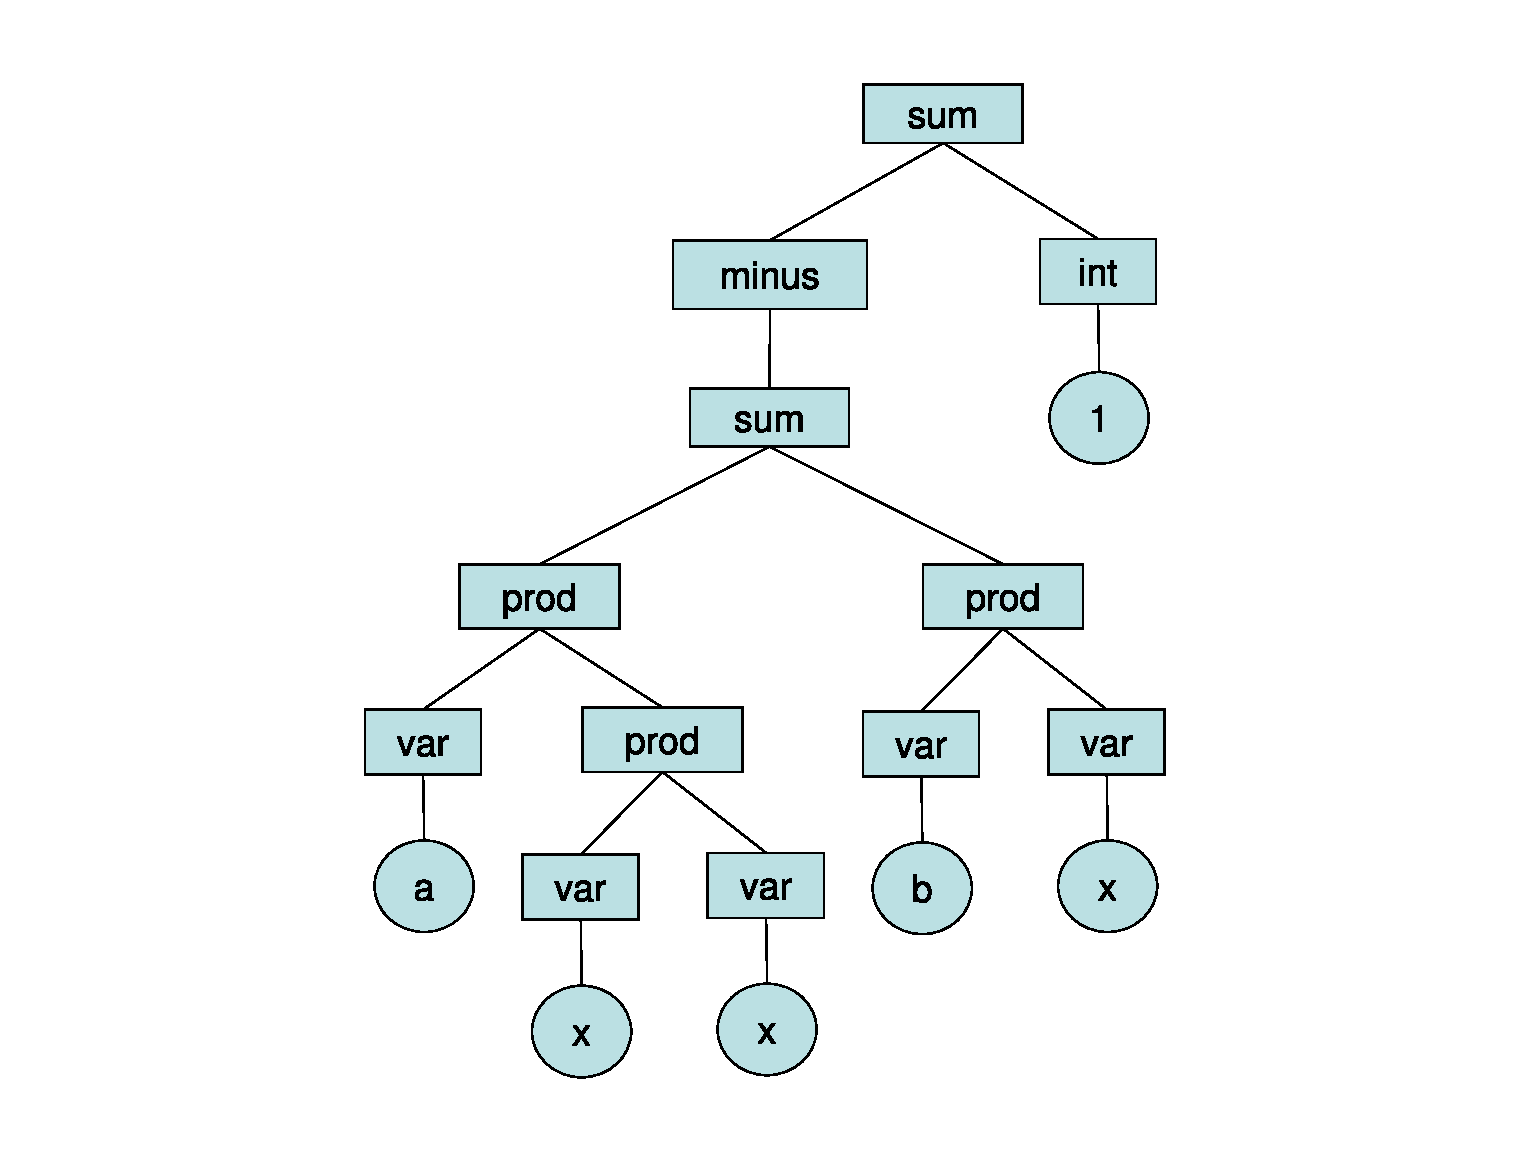
\includegraphics[width=5in]{parsetree}
\caption{Parse tree for $-(a(x\cdot x)+ bx) + 1$.}
\label{fig:parse}
\end{figure}

In a computer, such a tree would be represented by pairs or triples
that begin with a
\emph{tag} equal to the label of the top node of the parse tree.  
The general definition of parse trees for $\aexp$'s would be:

%\newcommand{\paexp}{\text{Aexp-parse-tree}}

\begin{definition}\label{arithparse}
The set $\paexp$ of \emph{parse trees for arithmetic expressions} 
over a set of
\emph{variables} $V$ is defined recursively as follows:
\begin{itemize}
\item \inductioncase{Base cases}:
\begin{enumerate}
\item If $n \in \integers$, then $\ang{\texttt{int}, n} \in \paexp$.
\item If $v \in V$, then $\ang{\texttt{var}, v} \in \paexp$.
\end{enumerate}
\item \inductioncase{Constructor cases}: if $e,e' \in \paexp$, then
\begin{enumerate}
\item $\ang{\texttt{sum}, e, e'} \in \paexp$,
\item $\ang{\texttt{prod}, e, e'} \in \paexp$, and
\item $\ang{\texttt{minus}, e} \in \paexp$.
\end{enumerate}
\end{itemize}
\end{definition}

So the $\paexp$ corresponding to formula~\ref{ax} would be:
\begin{equation}\label{axtag}
\begin{array}{rll}
\left< \right. \texttt{sum}, 
         & \left< \right. \texttt{minus},\ \ \left< \right. \texttt{sum},
               & \ang{\texttt{prod},\ \ \ang{\texttt{var},\ a},
                                     \ang{\texttt{prod},\ \
                                            \ang{\texttt{var},\ x},\
                                            \ang{\texttt{var},\ x}}},\\
                               && \left. \left. \ang{\texttt{prod},\ \
                                       \ang{\texttt{var},\ b},\
                                       \ang{\texttt{var},\ x}}
                                   \right> \right>,\\
         & \left. \left. \ang{\texttt{int},\ 1} \right> \right>
\end{array}
\end{equation}
Now the expression~\ref{ax} is certainly a lot more humanly
intelligible than~\ref{axtag}, but~\ref{axtag} is in the
representation best suited and commonly used in compiling and
processing computer programs.

\end{editingnotes}

\endinput

